% !TEX root =../main.tex

\chapter{Theoretischer Hintergrund und Konzepte}


\section{Definition Social Network}

% TODO: Zitate überprüfen. Groß- und Kleinschreibung sowie Satzzeichen scheinen nicht korrekt zu sein.

Nach \textcite[S. 2]{aggarwal:sn} \glqq in general, a social network is defined as a network of interactions or relationships, where the nodes consist of actors, and the edges consist of the relationships or interactions between these actors.\grqq \textcite{aggarwal:sn} meint \glqq the concept of social network is not restricted to the specific case of an internet- based social network such as Facebook, such interactions may be in any conventional or non-conventional form, whether they be face to face interactions, telecommunication interactions, email interactions or postal mail interactions\grqq


\section{Welche Konzepte Sozialer Netzwerke können angewendet werden}

Soziale Netzwerke existierten, um die Bedürfnisse bestimmter Personen zu erfüllen. Sie können anhand ihrer Funktionen wie folgt klassifiziert werden.

\begin{description}
\item[Auf Basis menschlicher Interaktion:] Dazu zählen allgemeine Soziale Netzwerke wie Facebook und Myspace, berufliche Netzwerke wie LinkedIn oder Partnervermittlungen wie Parship.
\item[Auf Basis von Blog-Publishing und User-Attention Services:] Als Beispiele sind hierfür Twitter und Follow 5 zu nennen.
\item[Auf Basis von Content Sharing:] Netzwerke welche primär dem Teilen von Inhalten dienen sind beispielsweise Flickr, YouTube oder Delicious.
\item[Auf Basis von Echtzeit-Kommunikation:] Beispiele für soziale Netzwerke mit einem Fokus auf Echtzeit-Kommunikation sind WhatsApp und Skype.
\end{description}

\begin{itemize}
\item Bei der Echtzeit-Kommunikation gibt es viele Möglichkeiten Informationen zu versenden. Beispiele hierfür sind Text (Instant Messenging), Sprache oder Video. Die Vorteile sind, dass das Senden und Erhalten von Information nahezu ohne Verzögerung geschieht.
\item Die Akteure welche Facebook nutzen können unterschiedliche Ausprägungen besitzen. Bei einem Facebook Account kann es sich z. B. um einen persönlichen Account in Form einer persönlichen Seite handeln. Facebook kann aber darüber hinaus auch als Business-Homepage, kommerzielles Werbekonto oder Business-Management-Plattform genutzt werden, um Events, Aktivitäten und Veranstaltung zu organisieren, beziehungsweise Nachrichten zu kommunizieren.
% TODO: Quelle Chara C der Datei litertur.bib hinzufügen und hier referenzieren.
% TODO: Groß- und Kleinschreibung innerhalb des Zitats kontrollieren.
\item Expert Discovery in Networks ( Chara C, Social network data analytics, Seite 11) \glqq Social networks can be used as a tool in order to identify experts for a particular task. given the activities of candidates within a context, we first descaribe methods for ecaluating the level of expertise for each of them. Many complex tasks often require the collective expertise of more than one expert\grqq
% TODO: Quelle für Zitat hinzufügen.
\item \glqq social Tagging:  much of the interaction between users and social networks occurs in the form of tagging, in which users attach short descriptions to different objects in the social network, such as images, text, video or other multimedia data.\grqq
\item Randoms walks and their Application in Social Networks. Ranking is one of the most well Kown methods in web search.Ranking Users in Social Networks with Higher-Order Structures:
\item 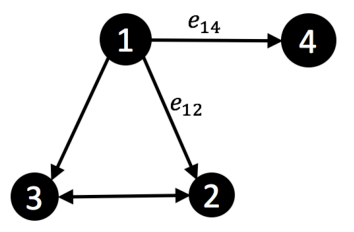
\includegraphics[width=0.3\textwidth]{bilder/social-network-users.png}
\item Nutzer 1 folgt bei dem dargestellten Sozialen Netzwerk  gleichzeitig den Nutzern 2, 3 und 4. Allerdings existieren hier Unterschiede. Nutzer 1 wird Nutzer 2 mehr als Nutzer 4 vertrauen. Der Grund dafür liegt darin, dass ein Nutzer dem Nutzer 1 folgt, ebenfalls dem Nutzer 2 folgt. Auf der Gegenseite kann Nutzer 4 keine weiteren Nutzer vorweisen, die ihm folgen.
% TODO: Gewünschte Aussage der folgenden Abschnitte muss herausgearbeitet werden. Im Moment leider schwer zu verstehen.
\item import application is to suggest  friends to a newcomer, z .B Netflix   is movie and music recommendation systems, where an user is suggested new movies and music basied on his or her rationgs so far.
% TODO: Quelle in literatur.bib eintragen und hier referenzieren.
\item Node (User) classification in social Networks. particular product , and it may be desirable to use the attribute and structural information in the network in order to learn other nodes which may also be interested in the same product. social networks als contain rich information about the content and structure of the network, which may be leveraged of this purpose.( Laut Charu C Seite 10 . an Introduction) z.B.  Zwei Nutzer sind miteinander in einem Socialnetwork verbunden. Es ist wahrscheinlich, dass die Knotenbeschriftungen ebenfalls korreliert sind.
\item Interaktionen führen dazu, dass verschiedene Akteure sich in ihrem Verhalten gegenseitig zu beeinflussen. Ein klassisches Beispiel dafür wäre eine virale Marketing Kampagne, bei der wir die Nachrichten zwischen miteinander verbundenen Teilnehmern in einem sozialen Netzwerk nutzen, um die Informationen über die verschiedenen Teile des Netzwerks zu verbreiten.
\item Intergrate real-time sensor- based content into dynamic social networks, accelerometers,mobile devices and other GPS-enabled devices, which can be used in a social setting for providing a dynamic and interactive experience
\end{itemize}


\section{Definition vom Social Media}

Laut \textcite[S. 8]{turban:sc} kann Social Media als Inhalt definiert werden, welcher durch Nutzer, mit Hilfe von Web 2.0 Plattformen, erzeugt wird. Das Erstellen dieser Inhalte dient hierbei laut \textcite[S. 8]{turban:sc} hauptsächlich dazu Meinungen, Erfahrungen und Erkenntnisse auszutauschen.


\section{Welche Konzepte von Social Media können angewendet werden}

\begin{itemize}
\item Verfolgt die Philosophie von miteinander verbundenen Personen \parencite[S. 8]{turban:sc}
\item Nutzer generieren, kontrollieren, nutzen und verwalten Inhalte zu geringen
oder keinen kosten \parencite[S. 8]{turban:sc}
\item Nutzer stellen den eigentlich bereitgestellten Wert bereit, während Betreiber lediglich eine Plattform anbieten, um dies zu ermöglichen ...
\item Geringe Barrieren für Nutzer, um sich an der Bereitstellung von Inhalten zu
beteiligen ...
\item Hohes Maß an Eigenverwaltung der Nutzer …
\end{itemize}


\section{Web 2.0}

Nach dem Platzen Dotcom-Blase im Herbst 2001 entstand die Frage, was erfolgreiche Internetunternehmen von den Unternehmen unterscheidet, welche aufhörten zu existieren. Die verbleibenden Internetunternehmen schienen zu einer neuen Generation des Internets zu gehören, welches sich konzeptionell grundlegend verändert hatte. Aus dieser Perspektive heraus wurde der Begriff des \term{Web 2.0} erschaffen.\\
\parencite{oreilly:web20}

Das Konzept des \term{Web 2.0} entstand hierbei in einer Brainstorming Sitzung zwischen O'Reilly and MediaLive International. Das Ergebnis dieses Brainstormings war die Erschaffung des Begriffs \term{Web 2.0} und die Gründung der \term{Web 2.0} Konferenz.\\
\parencite{oreilly:web20}

Tim O'Reilly, einer der Schöpfer des Begriffs \term{Web 2.0}, schrieb später, dass Menschen damit hadern, dass der Begriff \term{Web 2.0} nicht einfach definiert werden kann. \parencite{oreilly:levels-of-web20} Auch wenn der Begriff Web 2.0 nicht klar definiert werden kann, so soll er im Folgenden, soweit wie möglich eingegrenzt werden

Um herauszuarbeiten, was das \term{Web 2.0} von seiner vorherigen Generation unterschied definierte \textcite{oreilly:web20} die folgenden 7 Prinzipien.

\begin{enumerate}
	\item The Web As Platform
	\item Harnessing Collective Intelligence
	\item Data is the Next Intel Inside
	\item End of the Software Release Cycle
	\item Lightweight Programming Models
	\item Software Above the Level of a Single Device
	\item Rich User Experiences
\end{enumerate}

Diese Prinzipien definieren lediglich Themenschwerpunkte des \term{Web 2.0}, ermöglichen aber keine Möglichkeit zu erkennen, welche Webapplikationen dem \term{Web 2.0} angehören. \textcite{oreilly:levels-of-web20} führte hierfür ein System aus vier Ebenen ein. Anhand dieser vier Ebenen kann bestimmt werden, wie sehr eine Webapplikation den Prinzipien des \term{Web 2.0} entspricht.

\begin{description}
\item[Ebene 3] Anwendungen dieser Ebene sind am meisten auf das \term{Web 2.0} ausgerichtet. Sie existieren nur im Internet und leiten ihre Effektivität von der Vernetzung ihrer Nutzer ab. Ihre Effektivität wird durch Netzwerkeffekte gesteigert, welche sich verstärken, je mehr Leute die Anwendung nutzen. Beispiele für diese Art von Anwendungen sind Wikipedia und eBay.
\item[Ebene 2] Anwendungen der 2. Ebene können offline arbeiten, profitieren aber davon online verfügbar zu sein. Flickr ist ein Beispiel für eine solche Art von Anwendung. Sie profitiert von Photos, welche geteilt werden, und von einer, durch Nutzer erstellten, Tag-Datenbank.
\item[Ebene 1] Anwendungen der Ebene 1 funktionieren offline, erhalten aber zusätzliche Funktionalitäten wenn sie online betrieben werden. Ein Beispiel für eine Anwendung der Ebene 1 ist iTunes, da die Nutzer den integrierten Music-Store nur online nutzen können.
\item[Ebene 0] Diese Anwendungen funktionieren sowohl online als auch offline in exakt dem gleichen Maße. Google Maps ist ein Beispiel für eine Anwendung der Ebene 0.
\end{description}

Es ist darauf hinzuweisen, das für den Begriff \term{Web 2.0} weitere Eingrenzungen und Definitionen existieren. Im Rahmen dieser Arbeit wird der Begriff aber lediglich, wie durch \textcite{oreilly:web20} und \textcite{oreilly:levels-of-web20} beschrieben, verwendet.


\section{Definition von  e-Commerce}

Nach \textcite[S. 20]{merz:e-commerce} ist e-Commerce  \glqq die Unterstützung von Handelsaktivitäten über Kommunikationsnetze\grqq. E-Commerce ist der Einsatz von Kommunikationsprotokollen, Sicherheitsinfrastrukturen, digitalem Geld, Electrpmoc Shopping -malls und Datenaustausch….\grqq


\subsection{Welche Konzepte des eCommerce können angewendet werden}

\begin{description}
\item[Online Auktionen:] Aus \textcite[Kapitel 4: Wirtschaftliche Bedeutung von Ebay, S. 71]{hinneburg} \glqq da nicht die online -Auktionsmärkte selbst, sondern nur ihre Mitglieder Waren zum Verkauf anbieten, entscheidet die jeweilige Mitgliederzahl über die Quantität und Vielfalt des Warenangebotes eines Auktionsmarktes. Andererseits lohnt sich der Verkauf von Waren nur, wenn zahlreiche Käufer den Auktionsmarkt frequentieren.\grqq ~\textcite[S. 72]{hinneburg} hat noch konkret beschrieben, wie eine Auktion abläuft.

In Abbildung \vref{fig:laufende-auktionen} ist die Anzahl der laufenden Auktionen auf den zehn bedeutendsten deutschsprachigen Auktionsmärkten im Internet dargestellt.

\item[Gebrauchte Produkte verkaufen: ] Über Ebay Kleinanzeigen verkaufen viele Menschen Dinge, die sie nicht mehr benötigen – mit häufig äußerst kuriosen Anzeigen und witzigen Dialogen. Ein Verkäufer lädt ein Bild des Produkts mit entsprechenden Informationen wie Maßen und Preis hoch. Findet ein potentieller Käufer diese Anzeige interessant, tauschen sich Käufer und Verkäufer über weitere Details aus. In den meisten Fällen holt der Käufer das Objekt der Begierde beim Verkäufer ab. Beide Seiten profitieren, denn der Verkäufer hat wieder Platz in der Wohnung und bekommt Geld. Der Käufer hat für einen günstigeren Preis sein Wunschobjekt bekommen.

\item[Bewertungen von Produkten: ] Bei dem Online-Versandhändler Amazon kann man nach dem Kaufen eines Produktes eine Bewertung abgeben und Kommentare verfassen. Die Bewertung nutzt eine Skala von 1 - 5 Sternen und spiegelt die Zufriedenheit des Kunden wieder. Die Kommentare beschreiben konkret wie ein Käufer seine Kauferlebnis und das erworbene Produkt empfindet. Die Bewertung und Kommentare sind ein Teil der Dienstleistung, da sie anderen Nutzern helfen Produkte auszuwählen.
\end{description}

\begin{figure}
	\centering
	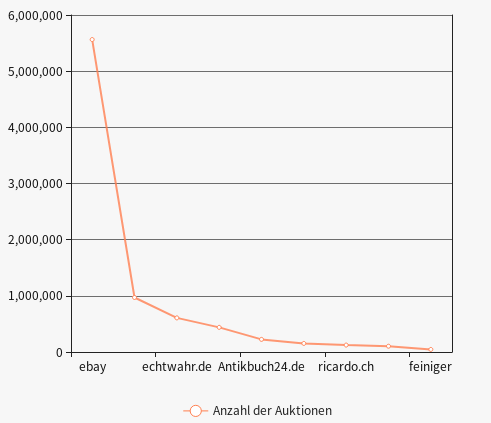
\includegraphics[width=0.7\textwidth]{bilder/laufende-auktionen.png}
	\caption[Laufende Auktionen]{Laufende Auktionen (Quelle: www.auktionssuche.de)}
	\label{fig:laufende-auktionen}
\end{figure}


\section{Social Commerce}

Social Commerce basiert auf den Konzepten von e-Commerce und Social Media. \textcite[S. 8]{turban:sc} beschreiben: \glqq{}The figur shows that social Commerce is created from the integration of e- Commerce and e-marketing using  Web 2.0/social Media applications.\grqq{} Es nutzt soziale Netzwerke, wie z.B. Twitter, BLOG oder Youtube, um Produkte durch soziale Interaktionen und vom Benutzer bereitgestellte Inhalte zu bewerben. Es ist ein effektiver Werbekanal für e-Commerce.


\subsection{Welche Konzepte von Social Commerce können angewendet werden}

\begin{itemize}
\item Die Einkaufsnachfrage des Nutzers entsteht unter dem Einfluss von anderen Nutzern. Es besteht eine starke Korrelation zwischen den Bedürfnissen eines Nutzers und den Bedürfnissen anderer Nutzer. Word-of-mouth (WOM) advertising (Marketing communication) is \glqq{}an unpaid form of promotion in which satisfied customers tell other people how much they like a business, product, or Service\grqq{}, \glqq{}Reaserch has revealed that customers are inclined to believe WOM rather than company generated promotions\grqq{} \parencite[S. 58]{turban:sc} Interesse und Wünsche werden mit denen von anderen Nutzern geteilt und durch Bewertungen, Kommentare oder Bilder angeregt.
% TODO: Aussage des Abschnitts noch nicht gut verständlich. Muss überarbeitet werden.
\item Sozial commerce leiten Nutzer an online shops,  der Einkaufsführer ist der Nutzer selbst. Es basiert auf der Erfahrung des Benutzers, Produktinformationen zu teilen, Produkte zu überprüfen, Produkte anzuzeigen und Produkte zu teilen, um mit anderen Nutzern zu interagieren und soziale Beziehungen mit sozialen Attributen herzustellen.
% TODO: Ist Viskosität hier das richtige Wort?
\item Die Plattform erstellt die Community. Sie bietet für viele Online-Shopping-Nutzerneinen Ort, um miteinander Einkaufsinformationen und Erfahrungen auszutauschen und gleichgesinnte kennenzulernen. Dadurch kann die Beziehung zwischen den Nutzern verstärkt werden. Die Viskosität des Benutzers und die Viskosität zwischen der Webseite und den Nutzern wird erhöht.

\begin{itemize}
\item Eine community-basierte Social Commerce -Plattform wie Facebook oder Twitter implementiert Präzisionsmarketing
\end{itemize}

\item Gewinnmodell: a, Werbung, 80\% Anteil; b, Kommission; c,  Mehrwertdienste, Sammeln von Beiträgen vom VI, um kostenpflichtige Dienste und spezielle Dienste zu erhalten; d,  Virtueller Warenverbrauch Plug-in-Anwendungsfreigabe von Drittanbietern
\item erweiterte Gewinnmodelle:

\begin{itemize}
\item Social Commerce kann Unternehmen helfen, Data Mining und Analyse von Benutzerpräferenzen und potenziellen Bedürfnissen durchzuführen und Online-Werbung für eine bestimmte Zielgruppe zu starten.
% TODO: Stichpunkt müssen geklärt und klarer formuliert werden. Sehr schwer zu verstehen.
\item Social Commerce kann kostenpflichtige Fragebogenumfragen anbieten und an Umfragen teilnehmen. Die Anzahl der Benutzer, die erhoben werden, um Unternehmen bei der Durchführung von professionellen Ermittlungen und Analysen zu unterstützen
\item Einführung des PPC- und Keyword-Bidding-Service und Einführung des SOLOMO-Modells. Solomo ist ein Akronym für Social Local Mobile ist die soziale, Lokalisierung und mobiles Internet zu verbinden. Kurz gesagt, das SOLOMO-Modell soll lokalisierte Dienste für Benutzer mit gemeinsamen Bedürfnissen über das Internet bereitstellen und effektiv online und offline integrieren.
\end{itemize}

\end{itemize}

Ein wichtiger Faktor im Social Commerce ist das Bild: Website-Betreiber stellen kostenlose, herunter-ladbare Software bereit, die es den Kunden erleichtert, Fotos hochzuladen und Einkaufserlebnisse auszutauschen. Eine solche Software ermöglicht es den Verbrauchern nicht nur, ihre Lieblingsprodukte aufzulisten, sondern auch die Fotos von Einkaufslisten anzupassen und eine Einnahmequelle zu schaffen. Zum Beispiel können diese Websites durch den Verkauf von Click-to-Pay-Anzeigen Geld verdienen. Sie können auch eigene marktrelevante Informationen anbieten.


\section{Welche Konzepte des Online Gamings können angewendet werden}

\begin{itemize}
\item Die Spielteilnehmer kooperieren, um eine Aufgabe zu erfüllen. Sie können ein Team bilden oder auch alleine eine Aufgabe erfüllen.
\item Die Spielszene ist ansprechend und detailliert.
% TODO: Bitte aussage dieses Stichpunkts deutlicher machen. Im Moment nur schwer zu verstehen.
\item Virtuelle Güter verkaufen,  einen gesperrte Kompetenzen geben, sind die Gewinnsquelle von der Spiel Entwicklungsfirma.
\item Es gibt Communities für Gamer, um Nachrichten zu veröffentlichen und Erfahrungen auszutauschen \parencite[S. 126]{warmelink}.
\end{itemize}


\subsection{Vergleich mit anderen beliebten Webshops}

Tabelle \vref{tab:variable-breite} enthält den Vergleich mit anderen beliebten Webshops.

\begin{table}[htbp]
\centering
\begin{tabular}{l l l l l l}
\toprule
Kriterien				& Amazon	& Ebay	& Alibaba	& Bandcamp	& Zalando\\
\midrule
Nutzer-Community		& nein		& nein	& ja		& ja		& nein\\
Online-Kommunikation	& nein		& ja	& ja		& nein		& nein\\
Vielfältige Produkte	& ja		& ja	& ja		& ja		& nein\\
Pay by others			& nein		& nein	& ja		& nein		& nein\\
Bewertungen				& ja		& nein	& ja		& ja		& ja\\
\bottomrule
\end{tabular}
\caption{Tabelle mit variabler Spaltenbreite}
\label{tab:variable-breite}
\end{table}
